\section{FuzzBench}
\label{sec:fuzzbench}

\subsection*{Fuzzer Benchmarking As a Service}

\say{FuzzBench is a free service that evaluates fuzzers on a wide variety of real-world benchmarks, at Google scale. The goal of FuzzBench is to make it painless to rigorously evaluate fuzzing research and make fuzzing research easier for the community to adopt.} \cite{metzman2020fuzzbench}

\begin{figure}[!t]
    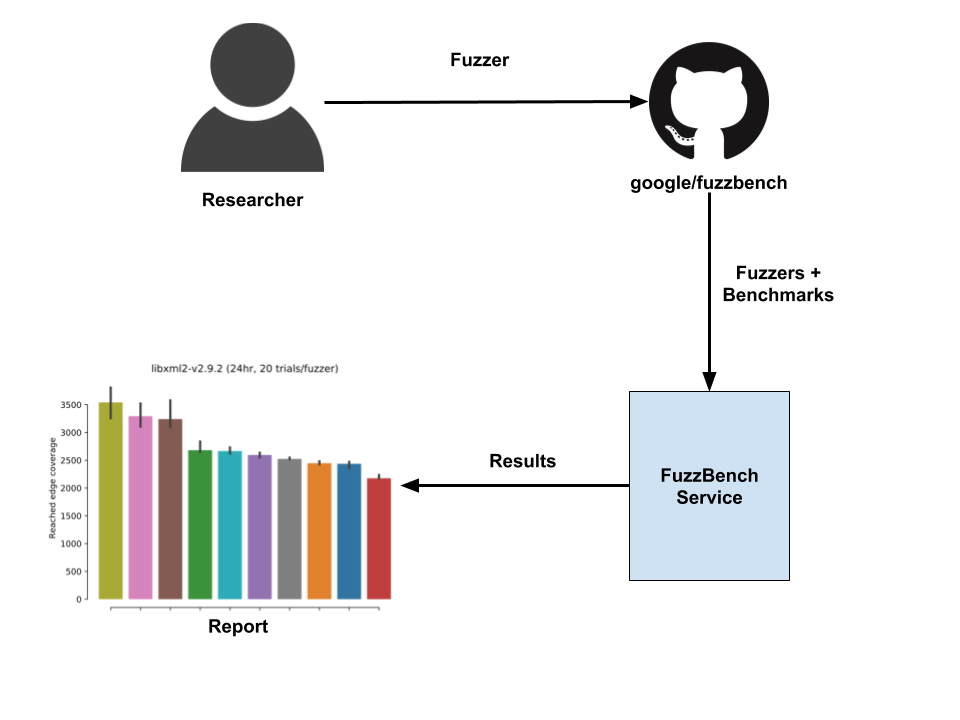
\includegraphics[width=\textwidth]{Chapter4/FuzzBench-service.png}
    \centering
    \caption{Fuzzbench overview}
    \label{fig:fuzz_bench}
\end{figure}

Of the main features of Fuzzbench, we use the following features to test Waffle:

\begin{itemize}
    \item \textbf{Fuzzer API:} An API for integrating fuzzers.
    \item \textbf{Custom/Standard benchmarks:} FuzzBench provides a set of real-world benchmarks. In addition, we can add our custom benchmarks or use any \textbf{OSS-Fuzz} project as a benchmark.
    \item \textbf{Reporting:} A reporting library is provided for generating graphs and statistical tests. These reports illustrate the performance of each fuzzer on different aspects. The evaluations are based on the stats such as the performance of fuzzers in finding unique vulnerabilities, or the growth and statistics of the code coverage during the experiments.
\end{itemize}

\subsection*{Add Waffle to FuzzBench}

The current version of FuzzBench contains more than 30 different fuzzers available for testing. To evaluate Waffle, we need to first add Waffle to the list of known fuzzers that FuzzBench could communicate with. FuzzBench requires three files to provide the instructions for introducing a fuzzer:

\begin{itemize}
    \item \texttt{builder.Dockerfile:} This file builds the fuzzer in a docker container. The recipe can be found in Appendix \ref{app:builder.docker}.
    \item \texttt{runner.Dockerfile:} This file defines the image that will be used to run benchmarks with Waffle.
\begin{lstlisting}[language=docker-compose,style=CodeStyle]
FROM gcr.io/fuzzbench/base-image
\end{lstlisting}  
    \item \texttt{fuzzer.py:} This file explains how to build and fuzz benchmarks using Waffle [Appendix \ref{app:fuzzer.py}].
\end{itemize}

According to the steps suggested for running an experiment, we add Waffle to FuzzBench, and we can assess if the fuzzer is working properly in the FuzzBench's environment.

\lstinputlisting[language=Bash,style=CommandStyle,label={code:run.sh},caption={Final steps for adding Waffle to FuzzBench}]{Codes/Chapter4/run.sh}

We faced some problems while adding Waffle, as the FuzzBench project \textbf{must} be built before the fuzzer is inserted into the \texttt{fuzzers} directory \cite{error0612}. Otherwise, \textbf{local experiments} would fail due to existing bugs.

\subsection*{Start an experiment}

There are three methods for initiating an experiment in FuzzBench:

\begin{itemize}
    \item \textbf{Request in FuzzBench} \say{The FuzzBench service automatically runs experiments that are requested by users twice a day at 6:00 AM PT (13:00 UTC) and 6:00 PM PT (01:00 UTC). \cite{request_exp}}
    \item \textbf{Setting up a Google Cloud Project:} We can run our experiment on \textbf{GCP} \cite{request_gcp}.
    \item \textbf{Run a local experiment:} We can start the experiment on a non-cloud platform as well. Running a experiment on a local computer may lack enough resources for running different tests in parrallel.
\end{itemize}

We use a \textbf{local experiment} for evaluations. The local computer runs on Ubuntu 18.04 64bits, with Intel® Core™ i7-3770 CPU @ 3.40GHz × 8, and 16 GBs of RAM. The measurements for the performance of HDD, show 30MB/s for reading from the disk, and can write for 25MB/s.
